\chapter{Funktionsweise traditioneller Compiler} \label{cha:3-Tradional_Compiler}

Der traditionelle Aufbau eines Compilers lässt sich mit folgendem Schema veranschaulichen:

\begin{figure}[h!]
    \centering
    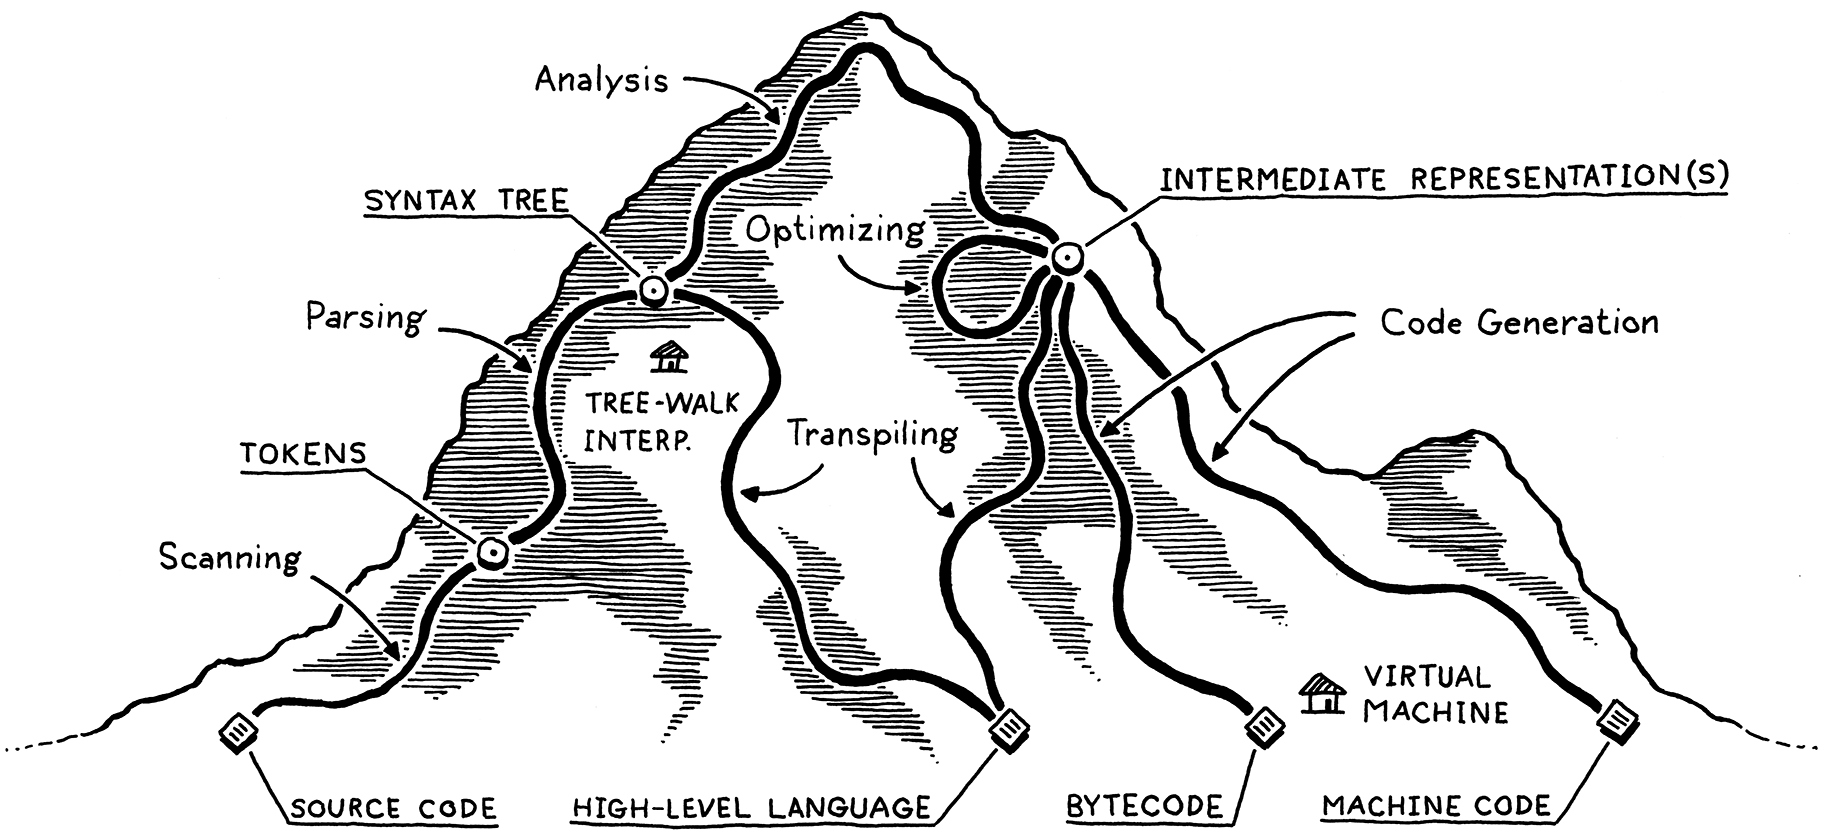
\includegraphics[scale=0.2]{resources/images/mountain.png}
    \caption[Schritte, die ein Compiler durchläuft (https://github.com/munificent/craftinginterpreters, besucht am 5.8.2024)]{Schritte, die ein Compiler durchläuft}
    \label{fig:mountain}
\end{figure}

In dieser Arbeit werde ich mich auf die in der unteren Abbildung \ref{fig:mountain-edited} dargestellten Schritte fokussieren.

\begin{figure}[h!]
    \centering
    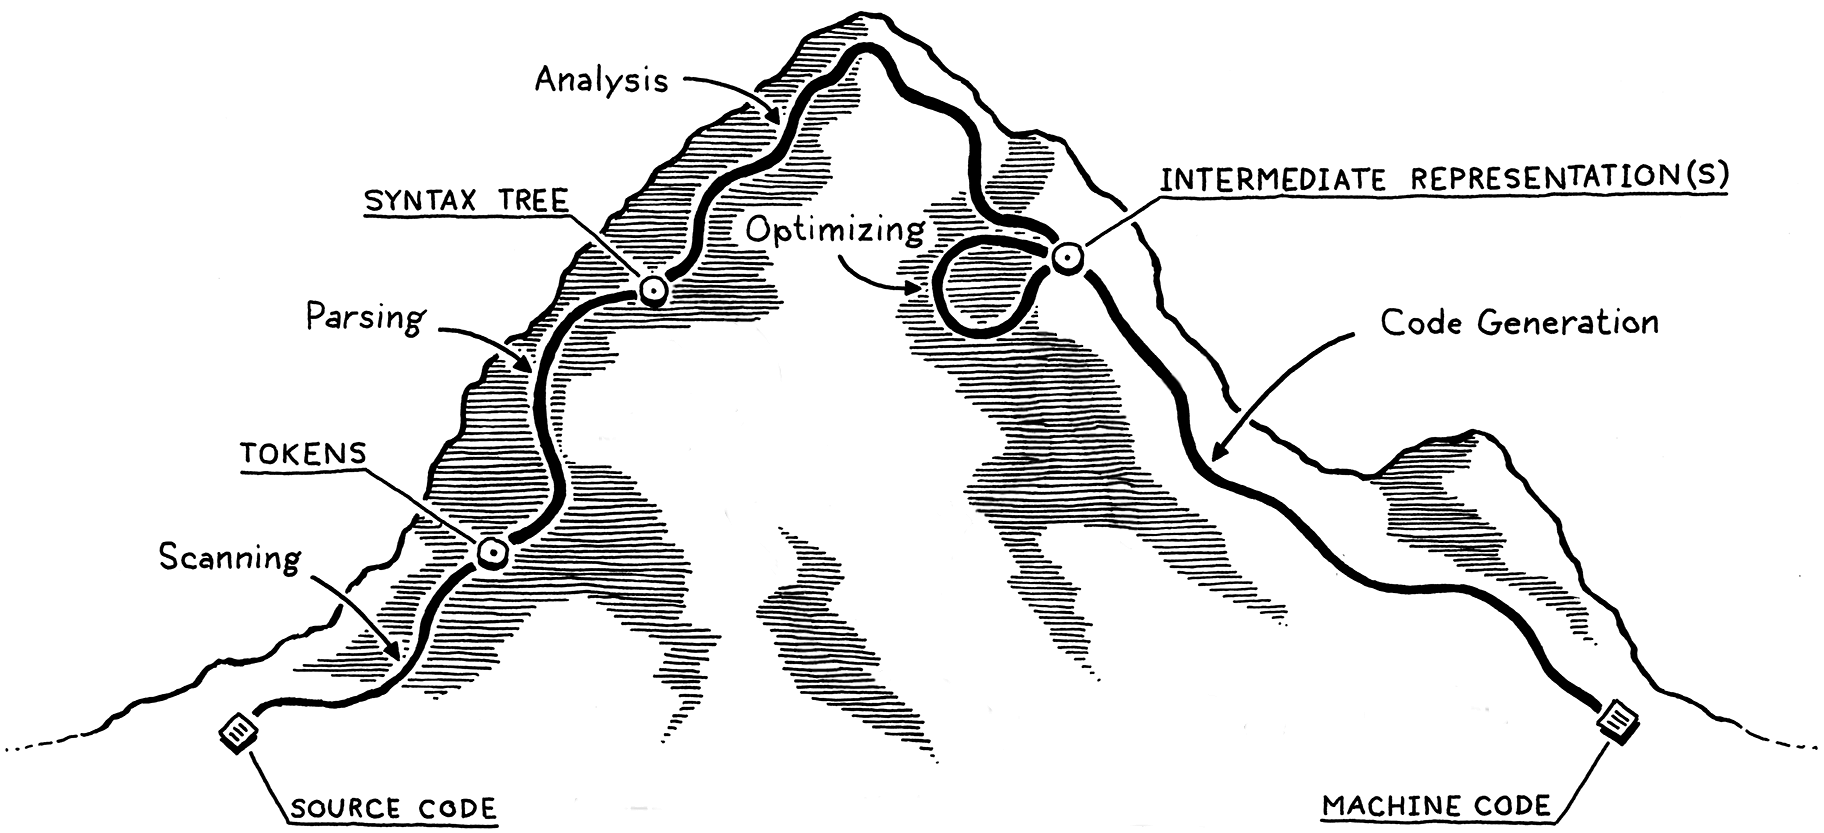
\includegraphics[scale=0.2]{resources/images/mountain-edited.png}
    \caption[Schritte, die in dieser Arbeit behandelt werden (Basierend auf Abbildung \ref{fig:mountain})]{Schritte, die in dieser Arbeit behandelt werden}
    \label{fig:mountain-edited}
\end{figure}

Die in dieser Maturaarbeit verwendeten Fachbegriffe entsprechen nicht immer denen aus Abbildung \ref{fig:mountain-edited}.
Bei der ersten Verwendung dieser Fachbegriffe wird jeweils die alternative aus Abbildung \ref{fig:mountain-edited} in Klammern angegeben.

Als Basis für diese Kapitel dienen die Quellen \cite{CompilersDragon} und \cite{Lecture}.

\section{Lexikalische Analyse (\textit{Scanning})}
Meist werden Programme so geschrieben, dass wir Menschen sie lesen und verstehen können. Dafür verwendet man Buchstaben, Zahlen, Sonderzeichen (wie + oder *) und Leerzeichen.
Diese Zeichen sind jedoch für den Computer nicht sofort verständlich. Der erste Schritt beim Kompilieren ist daher die lexikalische Analyse. Diese Analyse wird von einem Teil des Compilers, dem \textit{Lexer}, durchgeführt.
Die Aufgabe des \textit{Lexers} ist es, die Eingabedatei abzuarbeiten und die gefundenen Zeichen in sogenannte \textit{Tokens} zu verwandeln. Diese \textit{Tokens} sind Datenstrukturen, die der Compiler versteht und mit denen er weiterarbeiten kann.

Ein Beispiel der lexikalischen Analyse auf der Programmiersprache C:

\begin{lstlisting}[language=C, label=eg:preLex, caption=C code vor lexikalischer Analyse]
int foo()
{
    if (bar == 0)
    {
        return 0;
    }

    return 1;
}
\end{lstlisting}

\begin{lstlisting}[label=eg:postLex, caption=\textit{Tokens} nach lexikalischer Analyse]
Keyword         (keyword="int")
Identifier      (id="foo")
LParenthesis
RParenthesis
Keyword         (keyword="if")
LParenthesis
Identifier      (id="bar")
Operator        (operator=ComparisonEqual)
LiteralInt      (value=0)
[...]
\end{lstlisting}

Der \textit{Lexer} legt fest, welche Zeichen die Eingabesprache enthalten darf und welche Bedeutung ihnen zugesprochen wird. So ist zum Beispiel im \textit{Lexer} festgelegt, dass ein + Zeichen als Addition interpretiert wird.
Genauso wie im Listing \ref{eg:postLex} {\listingFont\selectfont 'if'} als \textit{Keyword-Token} gesehen wird, lässt sich im \textit{Lexer} auch bestimmen, dass ein Wort wie {\listingFont\selectfont 'else'} als Keyword angesehen werden soll.

\section{Syntaktische Analyse (\textit{Parsing})}
Der Compiler hat nun die Zeichen der Eingabedatei in ein für ihn verständliches Format übersetzt.
Jedoch fehlt dem Compiler noch das Verständnis für die Syntax der Eingabe-Programmiersprache.
Die meisten High-Level Programmiersprachen weisen Syntaxregeln auf. Diese beinhalten, wie Funktionen und Variablen definiert werden oder mit welchen Präzedenzregeln \textit{Expressions} evaluiert werden.
In diesem Schritt führt der sogenannte \textit{Parser} die syntaktische Analyse durch.
Dabei werden die bei der lexikalischen Analyse gefundenen \textit{Tokens} ineinander verschachtelt und in einen sogenannten \textit{Abstract Syntax Tree} (AST) überführt.

\begin{figure}[H]
    \centering
    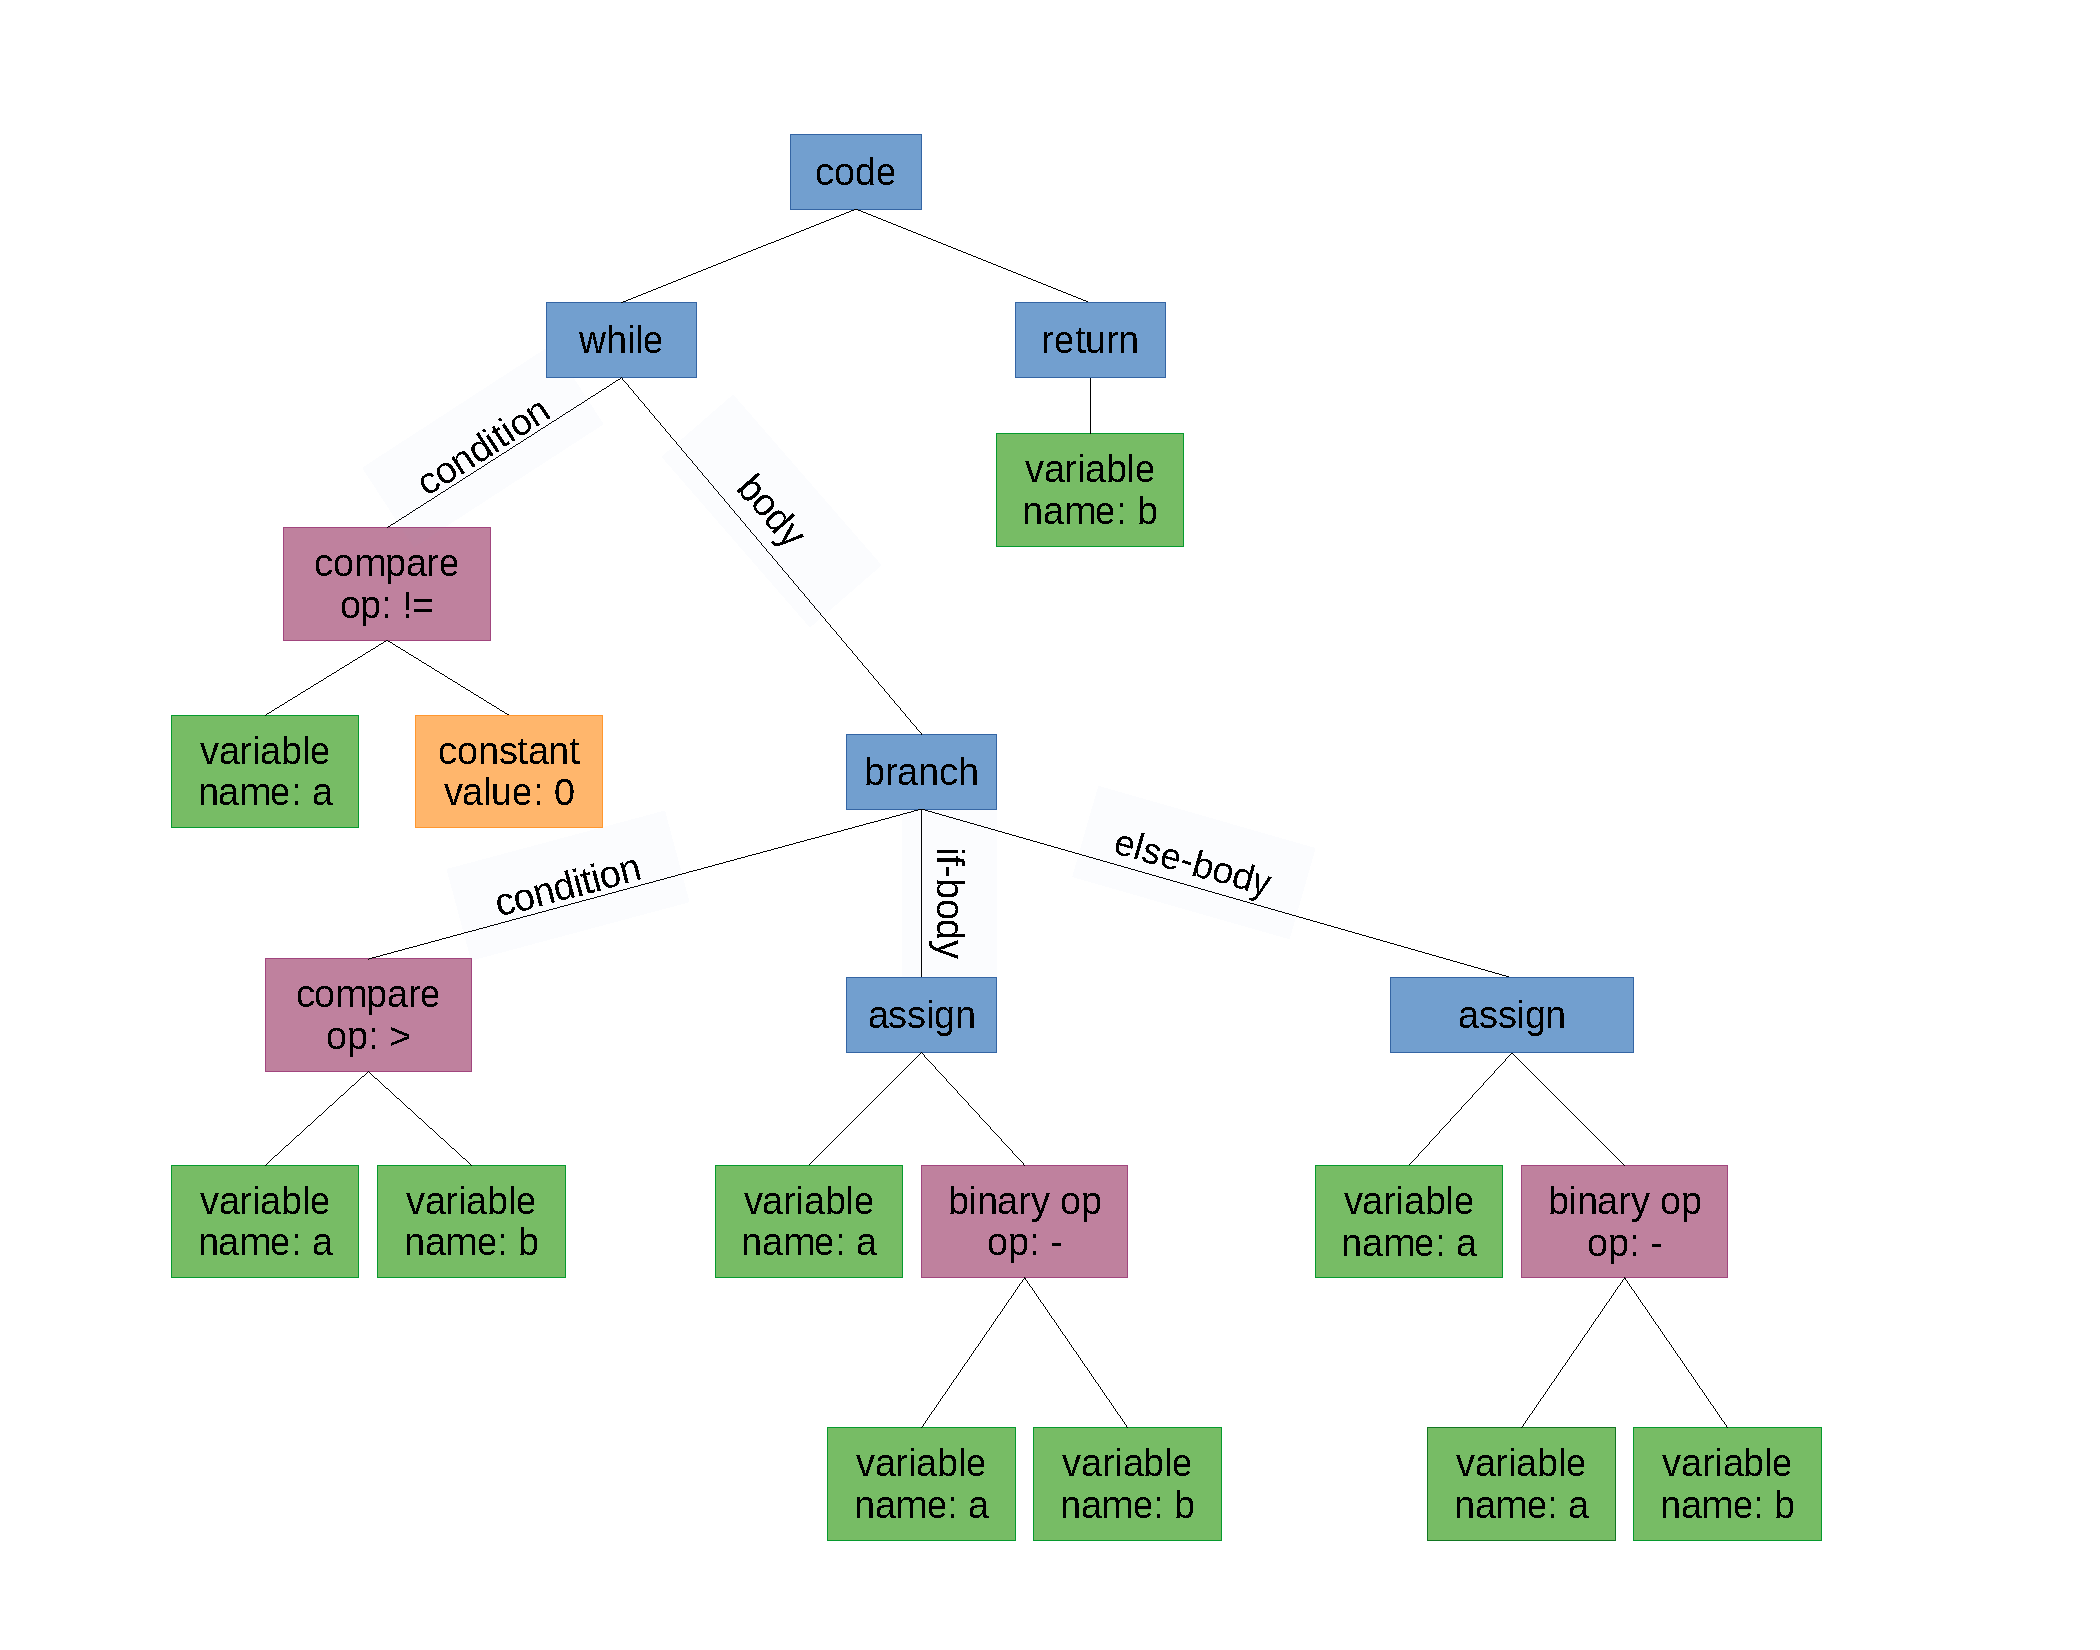
\includegraphics[scale=0.4]{resources/images/AST.pdf}
    \caption[AST zum euklidischen Algorithmus. (https://en.wikipedia.org/wiki/Abstract\_syntax\_tree, besucht am 5.8.2024)]{AST zum euklidischen Algorithmus}
    \label{fig:syntax-tree}
\end{figure}

Ein AST enthält somit nicht nur Informationen über die \textit{Tokens}, sondern über die gesamten Strukturen und Abhängigkeiten, die sich aus den \textit{Tokens} ergeben.
Variabel- und Funktionsdefinitionen oder komplexe \textit{Statements} und \textit{Expressions} sind im AST als \textit{Nodes} enthalten.
Wenn man die \textit{Nodes} des AST von unten nach oben durchquert, erhält man die Reihenfolge der einzelnen \textit{Tokens} ohne Abhängigkeitskonflikte.
Eine Subtraktion kann zum Beispiel erst ausgeführt werden, wenn sowohl die linke als auch die rechte Zahl bekannt ist.
Daher befindet sich, wie in Abbildung \ref{fig:syntax-tree} ersichtlich, die Subtraktion über den beiden benötigten Werten im AST.

\section{Semantische Analyse (\textit{Analysis})}
Semantik ist die Wissenschaft der Bedeutung von Wörtern einer Menschensprache. Bei einem Compiler geht es bei der semantischen Analyse nicht um die Bedeutung, sondern um die Korrektheit von \textit{Expressions}.
Wird eine Variable nicht konform ihres Datentyps verwendet, zum Beispiel wenn zwei Strings dividiert werden sollen, wird dies während der semantischen Analyse entdeckt und gemeldet.
Gegebenenfalls kann ein impliziter Cast, also ein automatischer Wechsel des Datentyps, hinzugefügt werden.
So geben zum Beispiel manche Programmiersprachen bei der Division zweier Ganzzahlen eine Fliesskommazahl zurück.
Auch werden unbekannte Variablen und Funktionen in diesem Schritt abgefangen.
Weiter wird der Datentyp einer \textit{Node} des AST an diese angebunden. Nach der semantischen Analyse sieht der AST aus Abbildung \ref{fig:syntax-tree} wie folgt aus:

\begin{figure}[H]
    \centering
    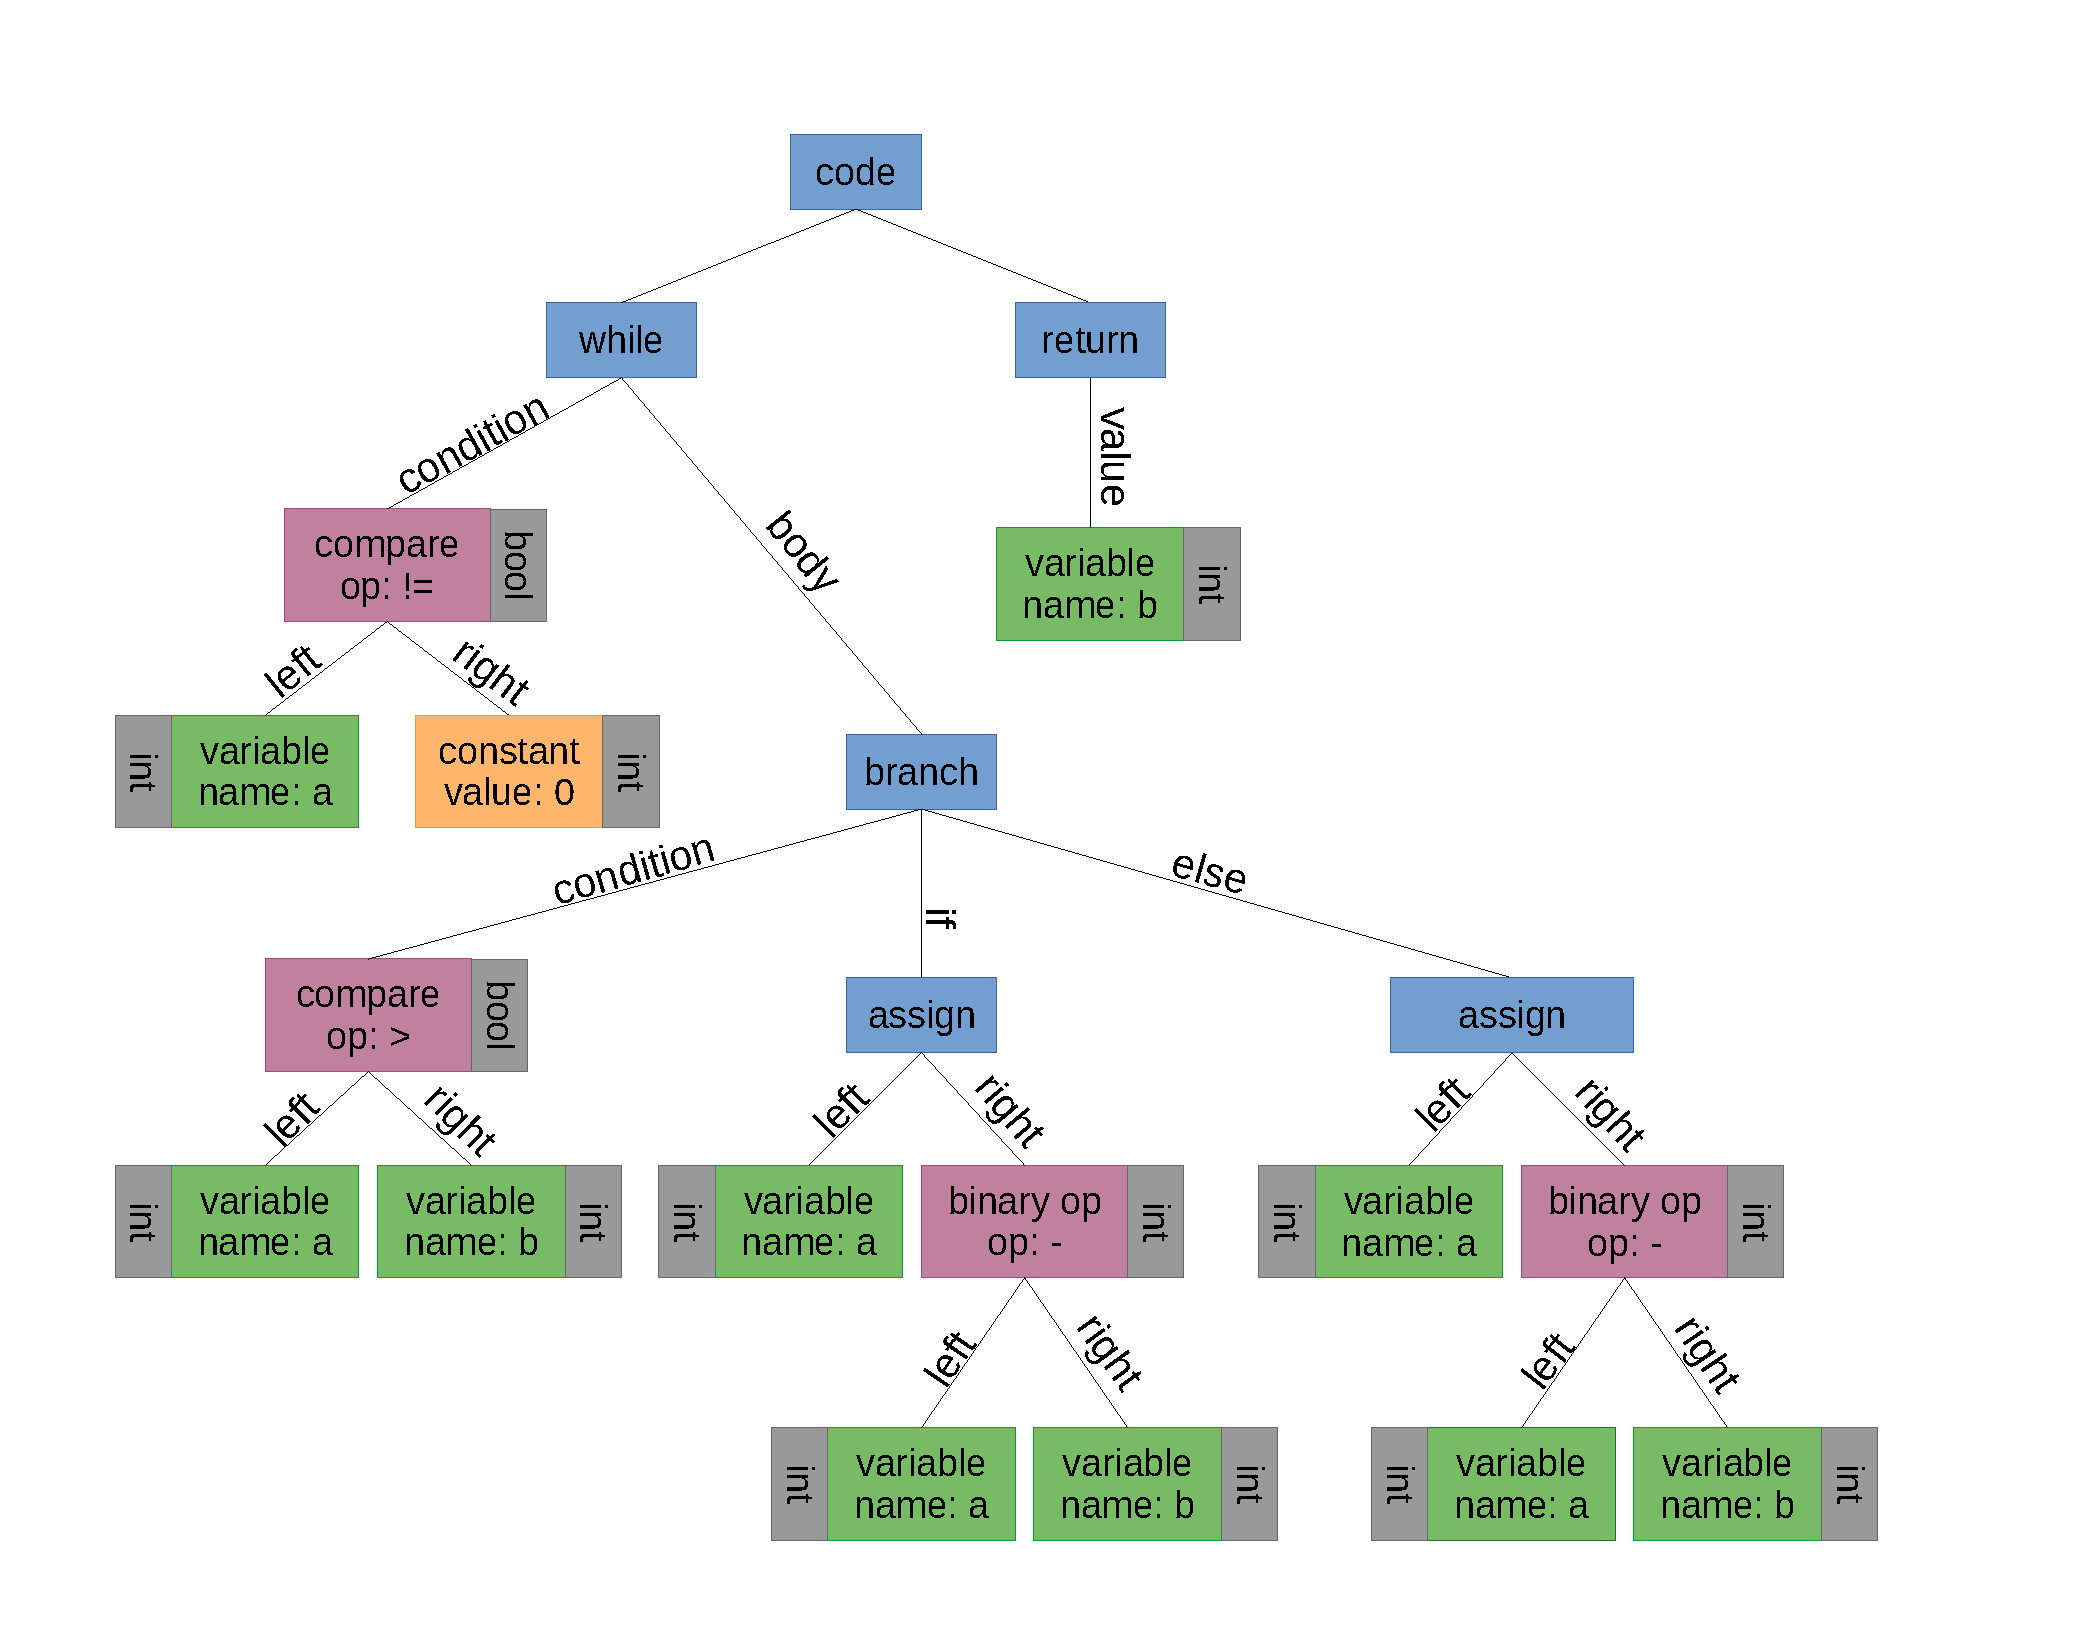
\includegraphics[scale=0.4]{resources/images/AST_with_types.pdf}
    \caption[AST nach der semantischen Analyse (Basierend auf Abbildung \ref{fig:syntax-tree})]{AST nach der semantischen Analyse}
    \label{fig:syntax-tree-with-types}
\end{figure}

Der AST wird nach der semantischen Analyse meist als Zwischencode (\textit{Intermediate Representation}) bezeichnet.
Da dieser Zwischencode in den weiteren Beispielen jedoch weiterhin dem Aufbau eines AST folgt, werde ich auch weiter AST als Begriff verwenden.


\section{Codegenerierung} \label{sec:traditional_code_generation}
Codegenerierung ist der finale und oft auch komplexeste Schritt, der ein Compiler ausführen muss.
Nun da die Eingabedatei als AST vorliegt, kann die Ausgabedatei generiert werden. Eine geläufige Methode der Codegenerierung ist die sogenannte \textit{Macro Expansion}.
Dabei wird der AST von unten nach oben schrittweise mit Teilen an Ausgabecode ersetzt.
Diese Ausgabecode-Teile sind häufig von den darunterliegenden \textit{Nodes} abhängig. Der AST aus Abbildung \ref{fig:syntax-tree-with-types} sähe nach erfolgreicher \textit{Macro Expansion} wie folgt aus:

\begin{figure}[H]
    \centering
    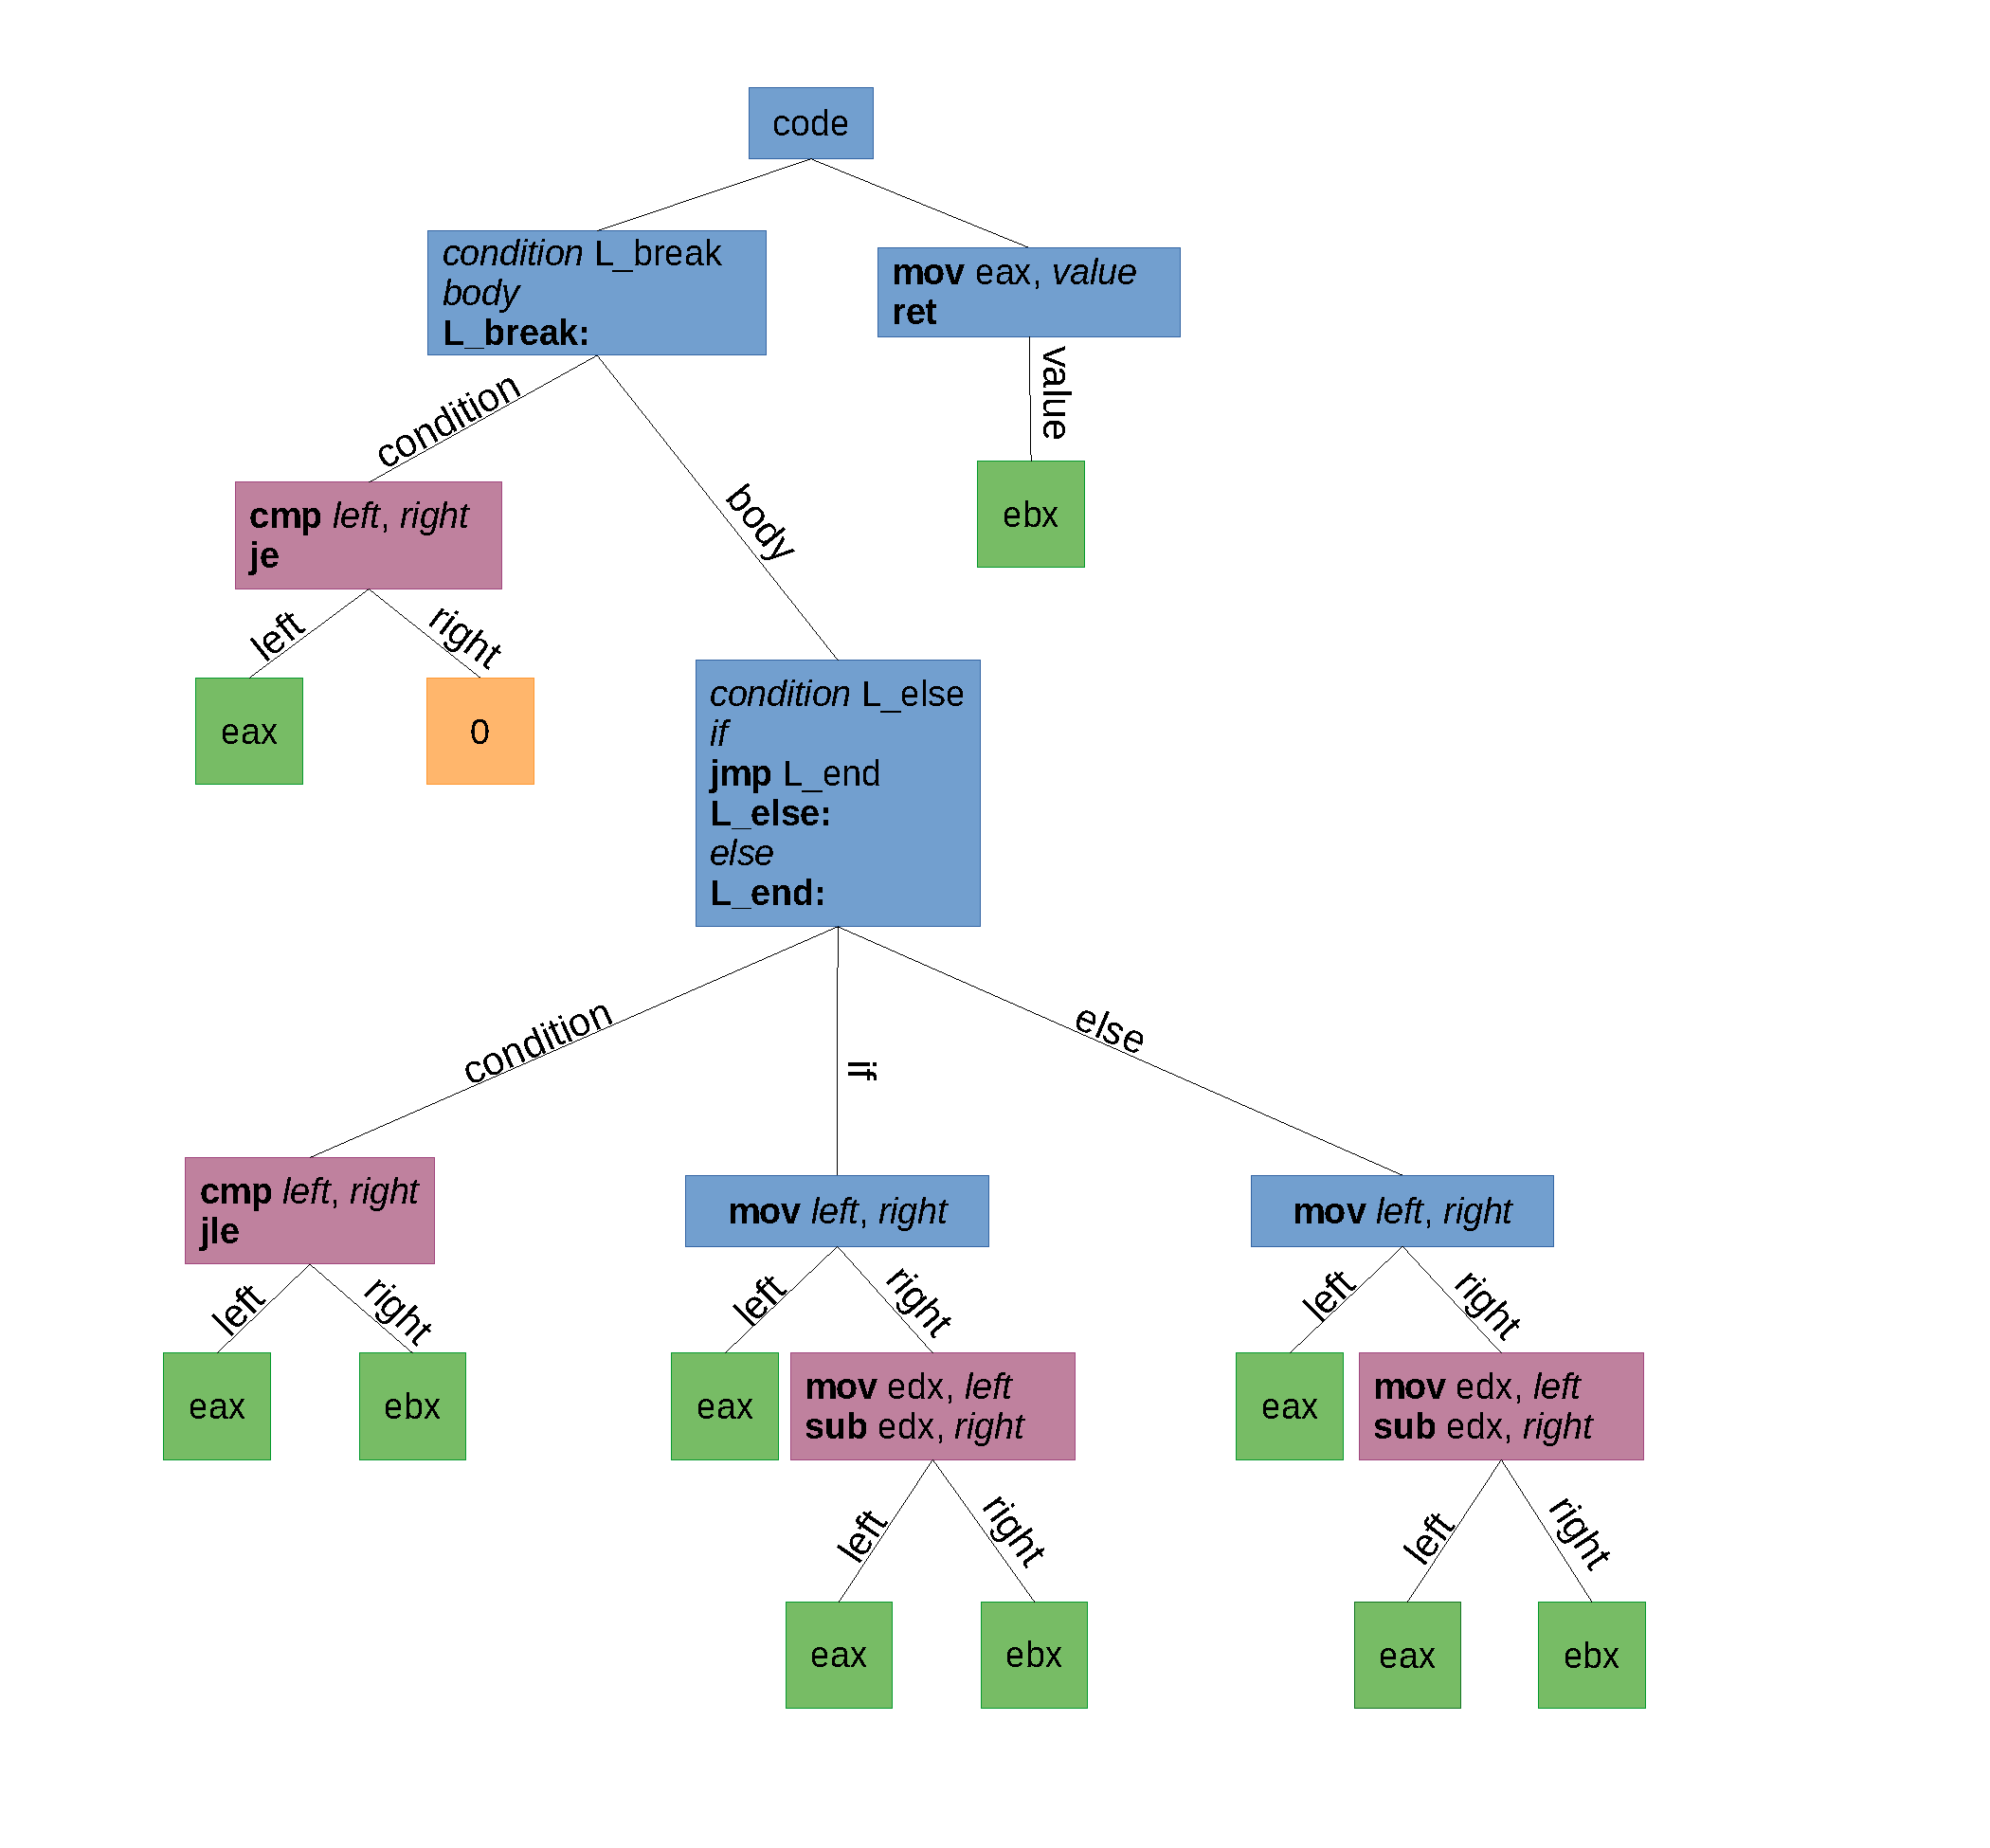
\includegraphics[scale=0.4]{resources/images/AST_macro_expansion.pdf}
    \caption[AST nach \textit{Macro Expansion}. (Basierend auf Abbildung \ref{fig:syntax-tree})]{AST nach \textit{Macro Expansion}}
    \label{fig:syntax-tree-after-macro-expansion}
\end{figure}

\section{Optimierung}
Codegenerierung ist zwar der letzte Schritt beim Kompilieren, trotzdem wurde eine wichtige Aufgabe des Compilers noch nicht betrachtet. Optimierung geschieht zwischen jedem der genannten Schritte und dies häufig mehrmals.
Dabei geht es darum die Ausgabedatei so effizient wie möglich zu machen. Effizient kann hierbei verschiedenes bedeuten.
Die Ausgabedatei muss so schnell wie möglich ausgeführt werden, Memory sparsam verwenden und dazu noch eine möglichst kleine Datei umfassen. 
Optimierungsmethoden reichen vom Überspringen der Kommentare und Umstellen von mathematischen Operationen, bis zum Entfernen von ungebrauchten Variablen und sogenannten \textit{Deadstores}.
Es muss von CPU-Registern profitiert, mit Heap-Arbeitsspeicher umgegangen und von Inlinefunktionen Gebrauch gemacht werden. % inline als deutsches Wort source: https://learn.microsoft.com/de-de/cpp/cpp/inline-functions-cpp?view=msvc-170
Optimierung ist also sehr vielseitig und komplex.
Wie Optimierung genau aussehen kann, wird daher in dieser Maturaarbeit nicht weiter betrachtet.
